\documentclass[a4paper, 11pt]{book}
\usepackage{comment} % enables the use of multi-line comments (\ifx \fi) 
\usepackage{lipsum} %This package just generates Lorem Ipsum filler text. 
\usepackage{fullpage} % changes the margin
\usepackage[a4paper, total={7in, 10in}]{geometry}
\usepackage[fleqn]{amsmath}
\usepackage[portuguese]{babel}
\usepackage{amssymb,amsthm}  % assumes amsmath package installed
\newtheorem{theorem}{Theorem}
\newtheorem{corollary}{Corollary}
\usepackage{graphicx}
\usepackage{cancel}
\usepackage{tikz}
\usetikzlibrary{arrows}
\usepackage{verbatim}
%\usepackage[numbered]{mcode}
\usepackage{titlesec}
\usepackage{float}
\usepackage{tikz}
\usepackage{tocloft}
\usepackage{standalone}
    \usetikzlibrary{shapes,arrows}
    \usetikzlibrary{arrows,calc,positioning}

    \tikzset{
        block/.style = {draw, rectangle,
            minimum height=1cm,
            minimum width=1.5cm},
        input/.style = {coordinate,node distance=1cm},
        output/.style = {coordinate,node distance=4cm},
        arrow/.style={draw, -latex,node distance=2cm},
        pinstyle/.style = {pin edge={latex-, black,node distance=2cm}},
        sum/.style = {draw, circle, node distance=1cm},
    }
\usepackage{xcolor}
\usepackage{mdframed}
\usepackage[shortlabels]{enumitem}
\usepackage{indentfirst}
\usepackage{hyperref}
\usepackage{etoolbox}
\usepackage{scalerel}
    
\makeatletter
\patchcmd{\chapter}{\if@openright\cleardoublepage\else\clearpage\fi}{}{}{}
\newcommand{\xRightarrow}[2][]{\ext@arrow 0359\Rightarrowfill@{#1}{#2}}
\makeatother

%\renewcommand{\thesubsection}{\thesection.\alph{subsection}}

\newenvironment{problem}[2][Problema] 
    { \begin{mdframed}[backgroundcolor=gray!20] \textbf{#1 #2} \\}
    {  \end{mdframed}}

% Define solution environment
\newenvironment{solution}
    {\textit{Solução:}}
    {}



\renewcommand{\qed}{\quad\qedsymbol}
%%%%%%%%%%%%%%%%%%%%%%%%%%%%%%%%%%%%%%%%%%%%%%%%%%%%%%%%%%%%%%%%%%%%%%%%%%%%%%%%%%%%%%%%%%%%%%%%%%%%%%%%%%%%%%%%%%%%%%%%%%%%%%%%%%%%%%%%
\begin{document}
%Header-Make sure you update this information!!!!
\noindent
%%%%%%%%%%%%%%%%%%%%%%%%%%%%%%%%%%%%%%%%%%%%%%%%%%%%%%%%%%%%%%%%%%%%%%%%%%%%%%%%%%%%%%%%%%%%%%%%%%%%%%%%%%%%%%%%%%%%%%%%%%%%%%%%%%%%%%%%
\large\textbf{Fernando Jorge} \hfill \textbf{Atividade - \#}   \\
Email: linguacavalcante@gmail.com \hfill Matrícula: 2021105189 \\
\normalsize Curso: PROFMAT - Geometria Plana MA-13 \hfill Semestre: 2021.2\\
Professor: Dr. José Carlos Almeida de Lima\hfill Data: $07^$ de Setembro de 2021 \\
\noindent\rule{7in}{2.8pt}

\chapter{Conceitos Geométricos Básicos}
\section{Introdução}
%%%%%%%%%%%%%%%%%%%%%%%%%%%%%%%%%%%%%%%%%%%%%%%%%%%%%%%%%%%%%%%%%%%%%%%%%%%%%%%%%%%%%%%%%%%%%%%%%%%%%%%%%%%%%%%%%%%%%%%%%%%%%%%%%%%%%%%%
% Problem 1
%%%%%%%%%%%%%%%%%%%%%%%%%%%%%%%%%%%%%%%%%%%%%%%%%%%%%%%%%%%%%%%%%%%%%%%%%%%%%%%%%%%%%%%%%%%%%%%%%%%%%%%%%%%%%%%%%%%%%%%%%%%%%%%%%%%%%%%%
\begin{problem}{1.1.3}
    \phantomsection
    \label{prob:1.1.3}
    Sejam \textit{A, B, C} e \textit{D} pontos de uma reta \textit{r}, tais que \textit{D} $\in$ $\overrightarrow{AC} \backslash AC$, \textit{B} $\in$  $\overrightarrow{DC} \backslash CD$ e $\overline{AC} = \overline{BD}$. Prove que  $\overline{AB} = \overline{CD}$   
\end{problem}
\begin{solution}
    Sejam \textit{A, B, C} e \textit{D} pontos na reta \textit{r} de forma que \textit{D} $\in$ $\overrightarrow{AC}$ e \textit{D} $\notin$ $\overline{AC}$. Assim como \textit{B} $\in$  $\overrightarrow{DC}$ e  \textit{B} $\notin$ $\overline{CD}$ e  $\overline{AC} = \overline{BD}$, mostrada na figura \ref{fig:1.1.3}:     
    
    \begin{figure}[H]
        \centering
        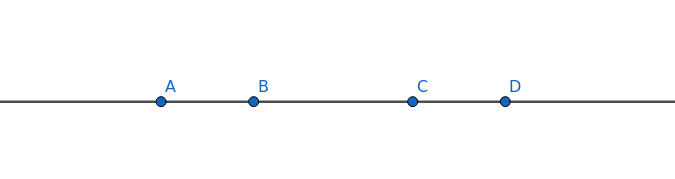
\includegraphics[scale=0.5]{imagens/1_1_3.png}
        \caption{Problema 1.1.3}
        \label{fig:1.1.3}
    \end{figure}

Podemos observar da figura acima que:
\[
    \overline{AC} = \overline{AB} + \overline{BC}
.\] 
\[
    \overline{BD} = \overline{BC} + \overline{CD}
.\] 
Do enunciado temos que $\overline{AB} = \overline{CD}$. Assim, realizando as substituições, temos:
\[
    \overline{AB} + \cancel{\overline{BC}} = \cancel{\overline{BC}} + \overline{CD}
.\] 
\[
    \overline{AB} = \overline{CD}
.\] 


\end{solution} 
\noindent\rule{7in}{2.8pt}\\

%%%%%%%%%%%%%%%%%%%%%%%%%%%%%%%%%%%%%%%%%%%%%%%%%%%%%%%%%%%%%%%%%%%%%%%%%
% Problem 2
%%%%%%%%%%%%%%%%%%%%%%%%%%%%%%%%%%%%%%%%%%%%%%%%%%%%%%%%%%%%%%%%%%%%%%%%%%%%%%%%%%%%%%%%%%%%%%%%%%%%%%%%%%%%%%%%%%%%%%%%%%%%%%%%%%%%%%%%

%%%%%%%%%%%%%%%%%%%%%%%%%%%%%%%%%%%%%%%%%%%%%%%%%%%%%%%%%%%%%%%%%%%%%%%%%
\begin{problem}{1.1.5}
    \phantomsection
    \label{prob:1.1.5}
Marque no plano, com o auxílio de uma régua e compasso, três pontos \textit{A, B} e \textit{C} tais que $\overline{AB} = 5cm$, $\overline{AC} = 6cm$ e $\overline{BC} = 4cm$.   
\end{problem}
\begin{solution}
    Ao construirmos os três segmentos de retas, com suas respectivas medidas, encontraremos duas soluções, o qual veremos a seguir os passos:
    \begin{enumerate}[\textbf{\arabic*}:]
        \item Iniciamos o problema desenhando três segmentos de retas $\overline{AB}$, $\overline{AC}$ e $\overline{BC}$ num plano qualquer, com comprimento respectivamente iguais a $5cm$,  $6cm$ e  $4cm$. Após isso marcamos o ponto A em qualquer lugar do plano.
        \item Chamaremos de $c_{ab}$ e  $c_{ac}$ as circunferências que possuem como centro o ponto  \textit{A} e raios respectivamentes iguais a $\overline{AB}$ e $\overline{AC}$, as desenhando-as. Dessa forma, os pontos \textit{B} e \textit{C} estão localizados nas linhas que delimitam as circunferências.
        \item A seguir, marcaremos um ponto B em qualquer lugar da circunferência $c_{ab}$ e construiremos o segmento de reta $\overline{AB}$ e observamos que é a medida do raio de $c_{ab}$, medindo $5cm$.
        \item Em seguida, traçamos a terceira circunferência $c_{bc}$ de centro no ponto \textit{B} e raio igual a $\overline{BC}$. Dessa forma, haverá dois pontos de intersseção entre a circunferência $c_{bc}$ e a circunferência $c_{ac}$, denominados ponto  \textit{C} e ponto $C_{1}$.
        \item A partir daí, observamos que o segmento $\overline{BC}$ é o raio da circunferência $c_{bc}$ e possui  $4cm$. Observamos também que o segmento  $\overline{AC}$ é o raio da circunferência $c_{ac}$ e possui  $6cm$. Dessa forma, foi construído problema, o qual está evidenciado na figura \ref{fig:1.1.5}. Como bônus, conseguimos perceber a outra solução, utilizando o ponto $C_{1}$.
    \end{enumerate}
 
    \begin{figure}[H]
        \centering
        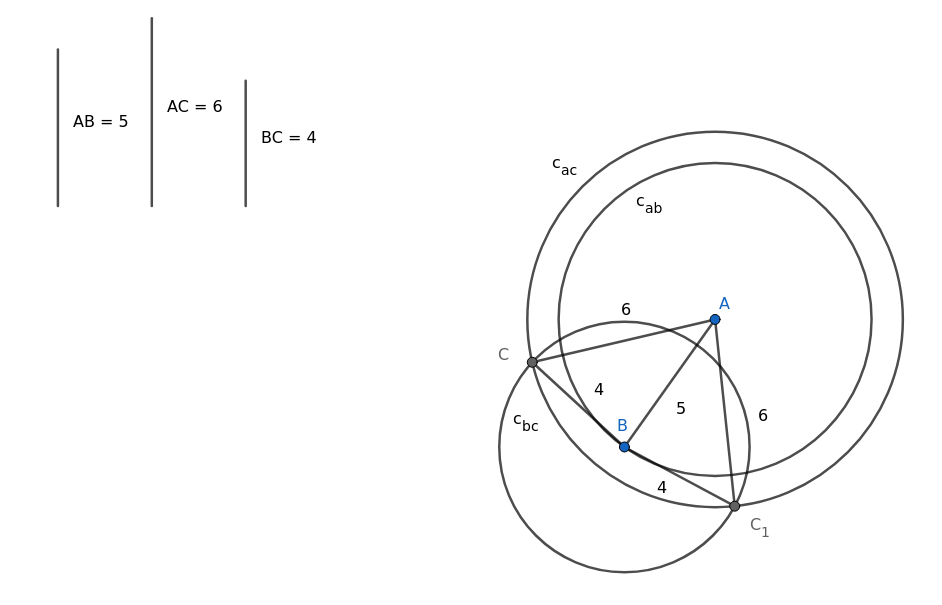
\includegraphics[scale=0.5]{imagens/1_1_5.png}
        \caption{Problema 1.1.5}
        \label{fig:1.1.5}
    \end{figure}
\end{solution}
    
\noindent\rule{7in}{2.8pt}
    
\section{Ângulos}

\begin{problem}{1.2.1}
    \phantomsection
    \label{prob:1.2.1}
Se a interseção de duas regiões convexas de um plano não for o conjunto vazio, prove que ela também é uma região convexa.
\end{problem}
\begin{solution}
    Se as regiões \textit{X} e \textit{Y} são convexas e a interseção entre elas não é vazio, então: \newline \newline
   Se \textit{X} é convexo, então $\forall A,B$ \in \textit{X} $\implies$ $\overline{AB}$ $\subset$ $X$, onde A e B são pontos quaisquer da região X. \newline 
   Se \textit{Y} é convexo, então $\forall A,B$ \in \textit{Y} $\implies$ $\overline{AB}$ $\subset$ $Y$, onde A e B são pontos quaisquer da região Y. \newline \newline
   Como $\overline{AB}$ $\subset$ $X$ e $\overline{AB}$ $\subset$ $Y$, então $\overline{AB}$ $\subset$ $X \cap Y$. E portanto, $X \cap Y$ é convexo.

\end{solution} 
\noindent\rule{7in}{2.8pt}\\

\begin{problem}{1.2.7}
    \phantomsection
    \label{prob:1.2.7}
    Cinco semirretas, de mesma origem \textit{O}, formam cinco ângulos que cobrem todo o plano e têm medidas em graus proporcionais aos números 2, 3, 4, 5 e 6. Calcule a medida do  maior de tais ângulos. 
\end{problem}
\begin{solution}
    Como os ângulos entre as semirretas cobrem todo o plano e tomando os ângulos entre elas por $\hat{a}$, $\hat{b}$, $\hat{c}$, $\hat{d}$ e $\hat{e}$, temos:
    \[
    \hat{a} + \hat{b} + \hat{c} + \hat{d} + \hat{e} = 360^\circ
    \] 
    Colocando os fatores de proporcionalidades, encontramos a seguinte equação:
    \[
    \frac{\hat{a}}{2} = \frac{\hat{b}}{3} = \frac{\hat{c}}{4} = \frac{\hat{d}}{5} = \frac{\hat{e}}{6} = k
    \] 
    onde k é o fator de proporcionalidade. Substituindo as equações de proporcionalidades na primeira equação, obtemos:
    \[
    2k + 3k + 4k + 5k + 6k = 360^\circ
    \] 
    \[
    k = 18^\circ
    .\]
    Dessa forma, o maior ângulo entre eles é aquele que tem fator de proporcionalidade 6. Resolvendo sua equação encontramos:
    \[
    \hat{e} = 6k= 6\cdot18^\circ = 188^\circ
    .\] 
\end{solution}
\noindent\rule{7in}{2.8pt}
\\

\begin{problem}{1.2.11}
    \phantomsection
    \label{prob:1.2.11}
    Três semirretas de mesma origem \textit{O} forma três ângulos que cobrem todo o plano. Mostre que ao menos um desses ângulos mede pelo menos $120^\circ$ e ao menos um mede no máximo $120^\circ$.
\end{problem}
\begin{solution}
    Como os ângulos entre as semirretas cobrem todo o plano e tomando o ângulo entre elas por $\alpha$,  $\beta$ e  $\gamma$, temos:
     \[
    \alpha + \beta + \gamma = 360^\circ
    .\] 
    Supondo $\alpha \le \beta \le \gamma$, teremos:
    \[
    \alpha + \alpha \le \alpha + \beta \le \alpha + \gamma \implies 2\alpha \le \alpha + \beta \le \alpha + \gamma \implies 2\alpha + \gamma \le \alpha + \beta + \gamma \le \alpha + 2\gamma \implies 2\alpha + \gamma \le 360^\circ \le \alpha + 2\gamma
    .\] 
    A partir daí obtemos duas inequações:
    \[
    2\alpha + \gamma \le 360^\circ \implies \gamma = 360^\circ - 2\alpha
    .\] 
    \[
    \alpha + 2\gamma \ge 360^\circ \implies \alpha \ge 360^\circ - 2\gamma
    .\] 
    Substituindo a primeira equação na segunda, obtemos:
    \[
        \alpha \ge 360^\circ - 2\cdot\left( 360^\circ - 2\alpha \right) 
    .\] 
    \[
    \alpha \ge 120^\circ
    .\] 
    Substituindo \alpha na equação 1, encontramos:
    \[
    \gamma \le 120^\circ
    .\] 
    Assim, provamos que de $\alpha$ obtemos ao menos um ângulo maior ou igual a $120^\circ$ e de $\gamma$ ao menos um ângulo menor ou igual a $120^\circ$.

\noindent\rule{7in}{2.8pt}

\section{Polígonos}

\begin{problem}{1.3.3}
    \phantomsection
    \label{prob:1.3.3}
    Três polígonos convexos têm números de lados iguais a três naturais consecutivos. Sabendo que a soma dos números de diagonais dos polígonos é de $133$, calcule o número de lados do polígono com maior número de diagonais.
\end{problem}
\begin{solution}
    Sabendo que o número de lados dos polígonos são consecutivos e que a soma das diagonais equivale a $133$, teremos
    \[
        D_{n} = \frac{n \cdot \left( n - 3 \right)}{2}
    .\] 
    \[
        D_{n + 1} = \frac{\left( n+1 \right)  \cdot \left( n - 2 \right)}{2}
    .\] 
    \[
        D_{n + 2} = \frac{\left( n+2 \right)  \cdot \left( n - 1 \right)}{2}
    .\] 
    \[
        D_{n} + D_{n+1} + D_{n+2} = 133
    .\] \\    
    Onde $D_{n}$ é o número de diagonais do polígono  $P_{n}$ e assim sucessivamente.
    Substituindo as três equações acima na equação da soma de diagonais, teremos:
    \[
    \frac{n \cdot \left( n - 3 \right)}{2} + \frac{\left( n+1 \right)  \cdot \left( n - 2 \right)}{2} + \frac{\left( n+2 \right)  \cdot \left( n - 1 \right)}{2} = 133
    .\] 
    \[
        n^2 - n - 90 = 0 \implies n = 10 \; ou \; \cancel{n = -9}
    .\] 
    Como o número de lados deve ser maior que 0, temos que $n = 10$, sendo descartado  $n = 9$.
    Para finalizar, o maior polígono é  $P_{n+2} = n + 2 = 10 + 2 = 12$
\end{solution}
\\\noindent\rule{7in}{2.8pt}

\chapter{Congruência de Triângulos}
\section{Os casos LAL, ALA, e LLL}


\section{Aplicações de Congruência}

\begin{problem}{2.2.1}
    \phantomsection
    \label{prob:2.2.1}
    Construa com régua e compasso as bissetrizes internas do triângulo ABC da figura \ref{fig:2.2.1}
    \begin{figure}[H]
        \centering
        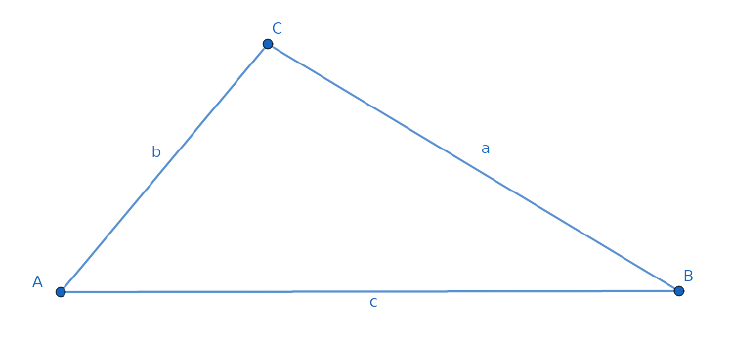
\includegraphics[scale=0.5]{imagens/2_2_1.png}
        \caption{bissetrizes internas de um triângulo}
        \label{fig:2.2.1}
    \end{figure}
\end{problem}
\begin{solution}
    Para construirmos uma bissetriz interna do ângulo $(\hat{A})$ seguiremos os passos a seguir:
    \begin{enumerate}[label=\textbf{\arabic*}:]
        \item  Construir um círculo de raio qualquer com centro no ponto A.
        \item  Marcar os dois pontos \textit{(D, E)}  de intersecção entre a circunferência e os segmentos de reta $\overline{AB}$ e $\overline{AC}$.
        \item Com o mesmo raio, traçar outras duas circunferências com centro nos pontos \textit{(E, F)}.  
        \item Marcar o ponto \textit{F} que intersecta as duas circunferências descritas no item 3.
        \item Finalizar construindo a semireta que inicia no ponto \textit{A} e passa pelo ponto \textit{P}, sendo denominada de bissetriz interna do ângulo $(\hat{a})$.  
    \end{enumerate}
    De forma análoga, construímos as outras duas bissetrizes internas, resultando na figura \ref{fig:2.2.1r}.
    \begin{figure}[H]
        \centering
        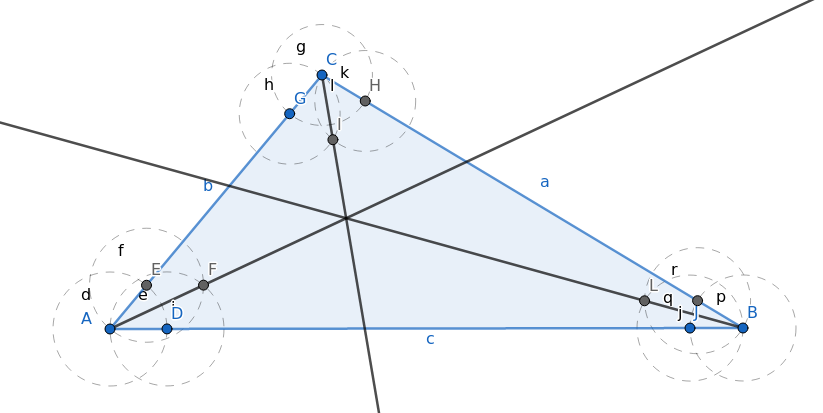
\includegraphics[scale=0.5]{imagens/2_2_1r.png}
        \caption{Problema 2.2.1}
        \label{fig:2.2.1r}
    \end{figure}
\end{solution}
\noindent\rule{7in}{2.8pt}\\

\begin{problem}{2.2.2}
    \phantomsection
    \label{prob:2.2.2}
    Construa com régua e compasso as medianas do triângulo \textit{ABC} da figura \ref{fig:2.2.2}
    \begin{figure}[H]
        \centering
        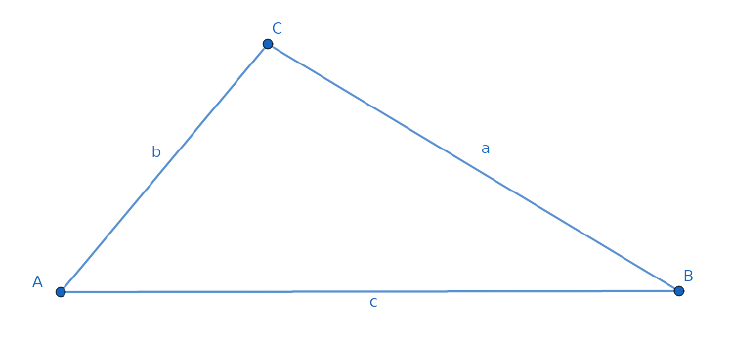
\includegraphics[scale=0.5]{imagens/2_2_2.png}
        \caption{medianas de um triângulo}
        \label{fig:2.2.2}
    \end{figure}
\end{problem}
\begin{solution}
    Para construirmos a mediana que parte do vértice \textit{A} e é relativa ao segmento $\overline{BC}$ devemos seguir os passos abaixo:
    \begin{enumerate}[\textbf{\arabic*}:]
        \item Construir a circunferência de raio maior que a média da medida do segmento $\overline{BC}$ com centro em \textit{B}. 
        \item Traçar a circunferência com mesma medida de raio do item 1, com centro em \textit{C}. 
        \item Marcar os pontos (\textit{D, E})  de intersecção entre as circunferências do item 1 e 2.
        \item Desenhar a mediatriz que passa pelos pontos \textit{(D, E)}. 
        \item Marcar o ponto médio \textit{M} do segmento  $\overline{BC}$, que é o ponto de intersecção entre a mediatriz do item 3 e o segmento de reta $\overline{BC}$. 
        \item Desenhar o segmento de reta que parte do ponto \textit{A} e termina no ponto \textit{M}, denominada mediana de A relativa a $\overline{BC}$. 
    \end{enumerate}
    De forma análoga, construímos as outras duas medianas, mostradas na figura \ref{fig:2.2.2r}.
    \begin{figure}[H]
        \centering
        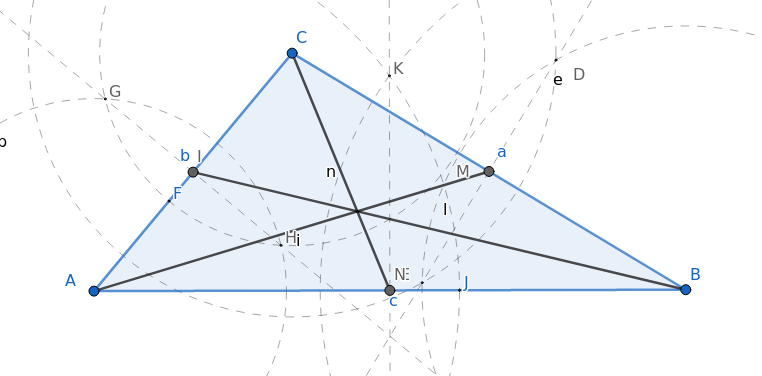
\includegraphics[scale=0.4]{imagens/2_2_2r.png}
        \caption{Problema 2.2.2}
        \label{fig:2.2.2r}
    \end{figure}
\end{solution} 
\noindent\rule{7in}{2.8pt}\\


\begin{problem}{2.2.6}
    \phantomsection
    \label{prob:2.2.6}
    Construa com régua e compasso o triângulo \textit{ABC}, conhecendo os comprimentos $\overline{AB} = c$, $\overline{AC} = b$ e $m_{a}$ da mediana relativa a  \textit{BC}.  
\end{problem}
\begin{solution}
    Para construirmos o triângulo devemos seguir os passos abaixo:
    \begin{enumerate}[\textbf{\arabic*}:]
        \item Devemos desenhar os três segmentos de retas com comprimentos iguais a \textit{c, b e $m_{a}$}.
        \item Marcamos o ponto \textit{A} em qualquer lugar do plano e em seguida traçamos a circunferência de raio $m_{a}$ e centro no ponto \textit{A}.  
        \item Marcamos o ponto \textit{M} em qualquer lugar da circunferência do item 2. 
        \item Em seguida, construímos outra circunferência de raio $m_{a}$ e centro no ponto \textit{M}. 
        \item Desenhamos a reta que passa pelo ponto \textit{A} e o ponto \textit{M}, esta reta conterá o segmento $\overline{BC}$.  
        \item Marcamos o ponto  \textit{$A_{1}$}, que é o ponto de intersecção entre a reta do item 5 e a circunferência do item 4.
        \item Traçamos duas circunferências de raio igual a \textit{c} de centros em \textit{A} e \textit{$A_{1}$}, o qual chamaremos respectivamente de \textit{$c_{ab}$} e \textit{$c_{1ab}$}.   
        \item Analogamente, traçamos duas circunferências de raio igual a \textit{b} de centros em \textit{A} e \textit{$A_{1}$}, o qual chamaremos respectivamente de \textit{$c_{ac}$} e \textit{$c_{1ac}$}.  
        \item Agora marcamos os pontos de intersecção \textit{B} e \textit{$B_{1}$} entre as circunferências \textit{$c_{ab}$} e \textit{$c_{1ac}$}, respectivamentes do lado esquerdo e do lado direito do ponto \textit{M}.  
        \item Dessa forma, encontramos o segmento $\overline{AB}$ do triângulo procurado.
        \item Analogamente, encontraremos o segmento $\overline{AC}$ refazendo os os itens
            \textit{8, 9 e 10} para as circunferências $c_{ac}$ e  $c_{1ab}$. 
        \item Por fim, traçamos o segmento de reta $\overline{BC}$, o qual possui como ponto médio \textit{M}, finalizando o triângulo ABC. 
    \end{enumerate}
    Podemos verificar a construção final na figura \ref{fig:2.2.6}.
    \begin{figure}[H]
        \centering
        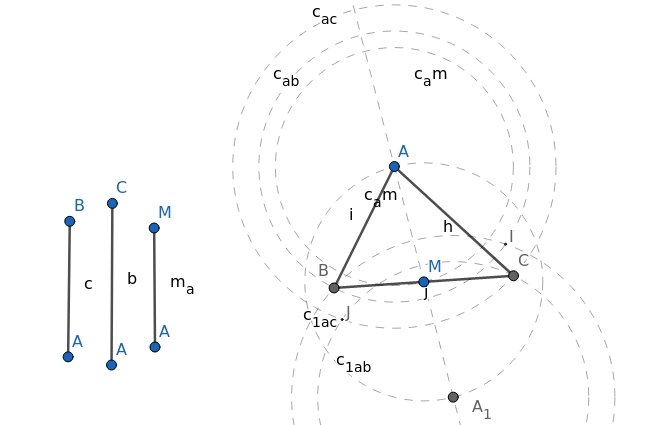
\includegraphics[scale=0.5]{imagens/2_2_6.png}
        \caption{Problema 2.2.6}
        \label{fig:2.2.6}
    \end{figure}
    
\end{solution}

\noindent\rule{7in}{2.8pt/\\

\begin{problem}{2.2.8}
    \phantomsection
    \label{prob:2.2.8}
    * Se \textit{ABC} é um triângulo isósceles de base \textit{BC}, prove que a bissetriz, a mediana e a altura relativas a \textit{BC} coincidem.   
\end{problem}

\begin{soluton}
    Dado um triângulo \textit{ABC} com base em $\overline{BC}$, traçaremos a bissetriz relativa ao lado \textit{BC}, evidenciada na figura \ref{fig:2.2.8}.  
    \begin{figure}[H]
        \centering
        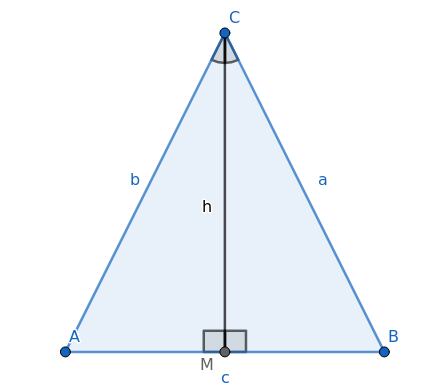
\includegraphics[scale=0.5]{imagens/2_2_8.png}
        \caption{Triângulo isósceles \textit{ABC} }
        \label{fig:2.2.8}
    \end{figure}
    Podemos observar da figura acima, que o triângulo \textit{ABC} isósceles, foi dividido em dois triângulos \textit{ACM} e \textit{BCM}. \\
    Observamos também que pelo caso LAL, os triângulos \textit{ACM} e \textit{BCM} são congruentes, pois:
    \[
    \begin{cases}
        \overline{AC} \equiv \overline{BC}, \mbox{ pois \textit{ABC é isósceles}}  \\
        \overline{CM}, \mbox{ é comum a ambos} \\
        \angle ACM \equiv \angle BCM, \mbox{ pois \textit{CM} é bissetriz}
    \end{cases} 
\xRightarrow{\textbf{LAL}}
\mbox{  \Delta ACM \equiv \Delta BCM}
    \]
    Dessa forma, verificamos que o ponto \textit{M} é ponto médio do segmento \textit{AB}, pois $\overline{AM} \equiv \overline{BM}$ e portanto, $\overline{CM}$ é também mediana relativa a $\overline{AB}$. \\
    Observamos também que o $\angle AMB$ é raso, possuindo então $180^\circ$ e concluímos:
    \[ 
    \angle AMC + \angle BMC = \angle AMB
    .\] 
    \[
    \angle AMC + \angle BMC = 180^\circ
    .\] 
    E como $\angle AMC \equiv \angle BMC$, temos:
    \[
    \angle AMC = \angle BMC = 90^\circ
    .\] 
    E portanto, o segmento $\overline{CM}$ é altura relativa a base $\overline{BC}$, pois os ângulos da base formam ângulos retos.
    Assim, o segmento de reta $\overline{AM}$ é bissetriz, mediana e altura relativa ao lado \textit{BC}. 
\end{soluton}

\noindent\rule{7in}{2.8pt}\\


\begin{problem}{2.2.10}
    \phantomsection
    \label{prob:2.2.10}
    * Seja $\Gamma$ um círculo de centro \textit{O} e \textit{AB} uma corda de $\Gamma$. Se \textit{M} é um ponto sobre \textit{AB}, prove que
    \[
    OM \perp AM \Leftrightarrow \overline{AM} = \overline{BM}
    .\] 
\end{problem}

\begin{solution}
    Nesse problema, podemos observar que haverá dois casos, mostrados a seguir:
    \begin{enumerate}[\textbf{Caso \arabic*}:]
        \item \textit{M} é ponto médio de \textit{AB}. \\\\
            Observando a figura \ref{fig:2.2.10}, podemos traçar os segmentos de retas $\overline{OA}$ e $\overline{OB}$ e verificar que estes segmentos correspondem ao raio do círculo. Assim o $\Delta OAB$ é isósceles com base  \textit{AB}. Como \textit{M} é ponto médio de \textit{AB}, o segumento \textit{OM} é mediana relativa a \textit{AB}. Portanto o segmento de reta \textit{OM} é perpendicular a base \textit{AB}, tendo sua prova vista no \nameref{sec:28}
            \begin{figure}[H]
                \centering
                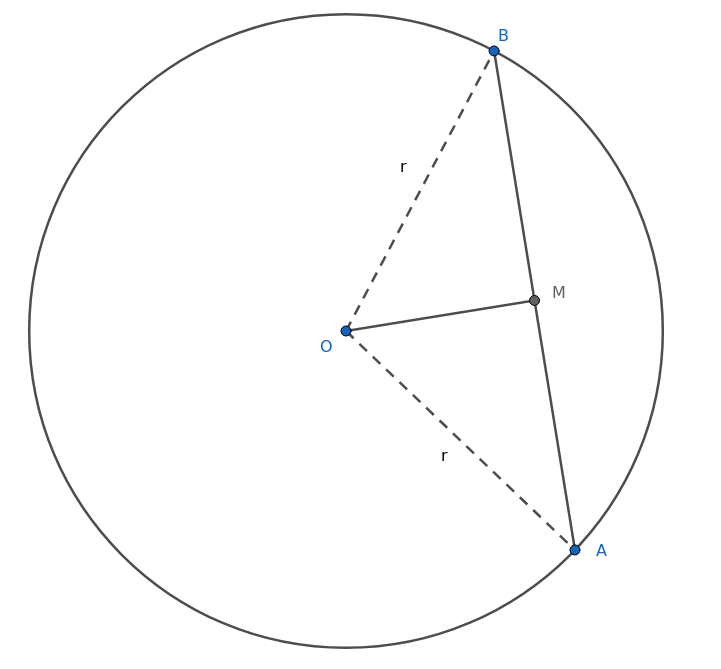
\includegraphics[scale=0.4]{imagens/2_2_10_1.png}
                \caption{Problema 2.2.10 - Caso 1}
                \label{fig:2.2.10}
            \end{figure}
        \item \textit{M} não é ponto médio de \textit{AB}. \\\\
            Observando a figura \ref{fig:2.2.10.2}, podemos traçar os segmentos de retas $\overline{OA}$ e $\overline{OB}$ e verificar que estes segmentos correspondem ao raio do círculo. Assim o $\Delta OAB$ é isósceles com base  \textit{AB}. Como observamos no \hyperref[prob:2.2.8]{Problem 2.2.8}, a altura relativa a base do triângulo isósceles é também mediana. Logo, para que o segmento de reta $\overline{OM}$ seja altura do triângulo, é preciso que \textit{M} seja ponto médio de \textit{AB}, o que neste caso não é, e assim $\overline{OM}$ não é altura do triângulo relativa a base \textit{AB}.    
            \begin{figure}[H]
                \centering
                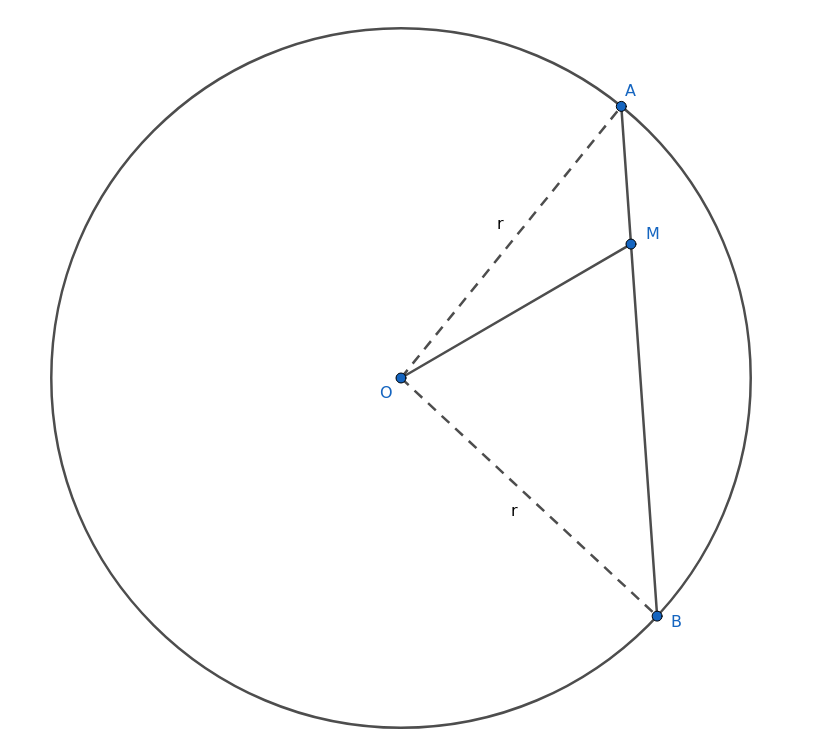
\includegraphics[scale=0.4]{imagens/2_2_10_2.png}
                \caption{Problema 2.2.10 - Caso 2}
                \label{fig:2.2.10.2}
            \end{figure}
    \end{enumerate}
    Assim, observando os dois casos, verificamos que:
    \[
    OM \perp AM \Leftrightarrow \overline{AM} = \overline{BM}
    .\] 
\end{solution}

\noindent\rule{7in}{2.8pt}

\section{Paralelismo}

\begin{problem}{2.3.2}
    \phantomsection
    \label{prob:2.3.2}
    * \textit{ABC} é um triângulo isósceles de base \textit{BC} e $D \in AB$,  $E \in AC$ são pontos tais que $\overleftrightarrow{DE} \parallel \overleftrightarrow{BC}$. Sendo \textit{F} o pontos de interseção dos segmentos \textit{CD} e \textit{BE}, mostre que $\overline{BF}=\overline{CF}$.       
\end{problem}
\begin{solution}
    Desenhando o esboço da figura \ref{fig:2.3.2} e observando que $\overline{DE} \parallel \overline{BC}$, podemos verificar utilizando o teorema de tales que o $\angle ADE = \angle ABC$ e o $\angle AED = \angle ACB$. Além do mais como o Triângulo \textit{ABC} é isósceles com base \textit{BC}, temos que $\angle ABC = \angle ACB$, e portanto, $\angle ADE = \angle ABC$ = $\angle AED = \angle ACB$.     
    \begin{figure}[H]
        \centering
        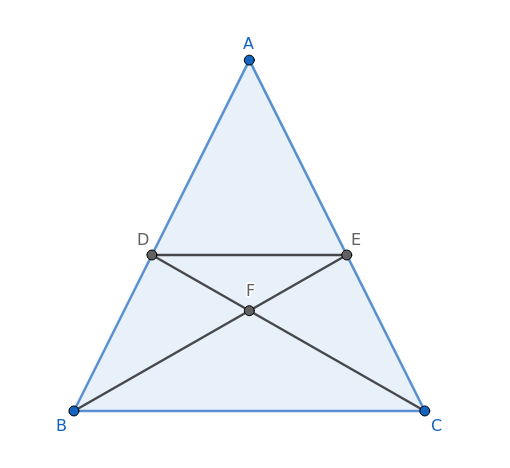
\includegraphics[scale=0.5]{imagens/2_3_2.png}
        \caption{Problema 2.3.2}
        \label{fig:2.3.2}
    \end{figure}
    
    Observamos também que pelo caso $LAL_{o}$, os triângulos \textit{ABE} e \textit{ACD} são congruentes, pois:
   \[
  \begin{cases}
      \overline{AB} \equiv \overline{AC} & \mbox{pois \textit{ABC} é isósceles} \\ 
      \angle A & \mbox{é comum a ambos} \\
      \angle ADE \equiv \angle AED & \mbox{pelo Teorema de Tales}
  \end{cases} 
  \xRightarrow{LLA_{o}}
    \Delta ABE \equiv \Delta ACD
   \]  
   Sendo assim, temos que $\angle DBF \equiv \angle ECF$ e os segmentos $\overline{AD} \equiv \overline{AE}$. De $\overline{AD} \equiv \overline{AE}$ é fácil perceber que $\overline{BD} = \overline{AB} - \overline{AD} = \overline{AC} - \overline{AE} = \overline{CE}$. Dessa forma, podemos verificar que os triângulos \textit{BDF} e \textit{CEF} são congruentes, pelo caso $LAA_{o}$, como verificasse a seguir: 
   \[
  \begin{cases}
      \angle DBF \ equiv \angle ECF & \mbox{pela congruência dos triângulos \textit{ABE} e \textit{ACD}  } \\ 
      \angle BFD \equiv \angle CFE & \mbox{opostos pelo vértice} \\
      \overline{BD} \equiv \overline{CE} & \mbox{vista acima}
  \end{cases} 
  \xRightarrow{LLA_{o}}
    \Delta BDF \equiv \Delta CEF
   \]  
   e portanto, $\overline{BF} = \overline{CF}$.
\end{solution}

\noindent\rule{7in}{2.8pt} \\

\begin{problem}{2.3.6}
    \phantomsection
    \label{prob:2.3.6}
    Na figura abaixo, prove que $r \parallel s \Leftrightarrow \alpha = \beta$ (os ângulos são denominados \textbf{correspondentes}).
    \begin{figure}[H]
        \centering
        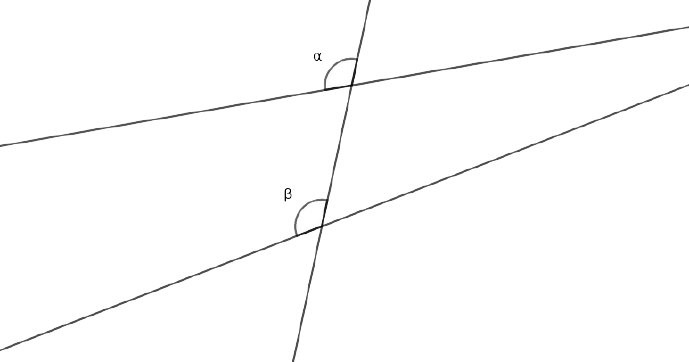
\includegraphics[scale=0.35]{imagens/2_3_6.png}
        \caption{Problema 2.3.6}
        \label{fig:2.3.6}
    \end{figure}
\end{problem}

\begin{solution}
    Vamos supor inicialmente que as retas não sejam paralelas e que $\alpha = \beta$, assim existirá um ponto C de interseção entre elas, formando o triângulo \textit{ABC} e posteriormente adicionamos o ponto médio (\textit{M}) do segmento \textit{BC}, formando os segmentos de reta \textit{AM}, $B_{1}M$, $AB_{1}$ e $B_{1}C$, como mostra a figura \ref{fig:2.3.6r}. 
    \begin{figure}[H]
        \centering
        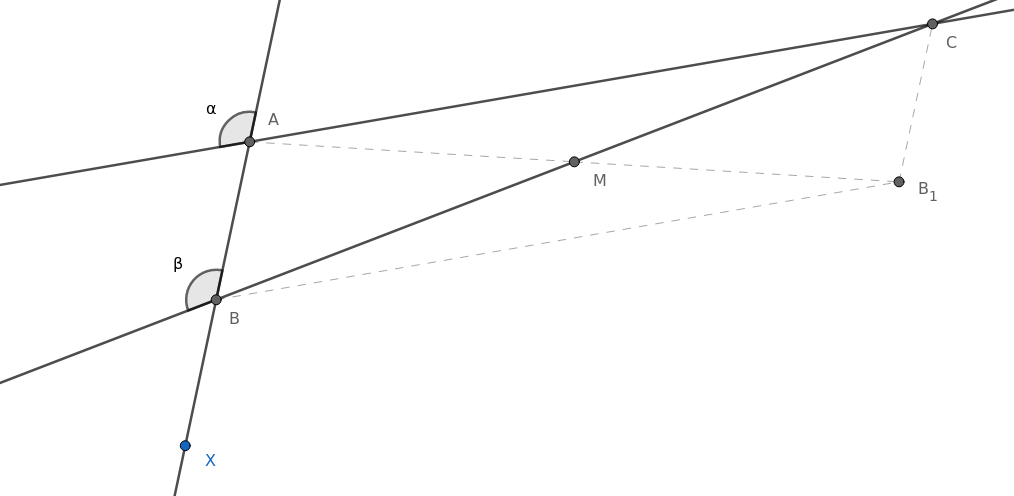
\includegraphics[scale=0.35]{imagens/2_3_6r.png}
        \caption{Problema 2.3.6}
        \label{fig:2.3.6r}
    \end{figure}
    Podemos observar da figura acima que $\beta$ é o ângulo externo do triângulo \textit{ABM} e $\alpha$ é ângulo interno do triângulo citado, pois $\alpha = \angle BAM$ (opostos pelo vértice). Assim, pelo teorema do ângulo externo, temos que $\beta > \alpha$, o que é um contradição pela hipótese e dessa forma,  $r \parallel s \Leftrightarrow \alpha = \beta$.   
\end{solution}

\noindent\rule{7in}{2.8pt} \\

\begin{problem}{2.3.11}
    \phantomsection
    \label{prob:2.3.11}
    * Dado um n-ágono convexo, faça os seguintes itens:
    \begin{enumerate}[label=(\alph*)]
    \item Prove que o polígono pode ser particionado em $n - 2$ triângulos, utilizando-se para tanto  $n-3$ diagonais que só se intersectam em vértices do mesmo.
    \item Conclua que a soma dos ângulos internos do polígono é  $180^\circ(n-2)$.
    \item Conclua que a soma de seus ângulos externos (um por vértice) do polígono é  $360^\circ$.
    \end{enumerate}
\end{problem}

\begin{solution}
    \begin{enumerate}
    \begin{enumerate}[(a)]
        \item 
    Seja \textit{P} um polígono convexo com \textit{n} vértices. Tomando um vértice qualquer $A_{1}$ por exemplo, temos que partindo de $A_{1}$, podemos formar $n-1$ segmentos, dos quais, os segmentos $A_{1},A_{2}$, $A_{2}A_{3}$ e $A_{n}A_{1}$ são lados de \textit{P}. Os $n-3$ segmentos restantes são diagonais de \textit{P}. \\
    Seja agora \textit{T} o número de triângulos de \textit{P}, partindo de $A_{1}$. Por Indução em  \textit{n}, temos que para $n=4$, são formados  $4-2=2$ triângulos. \\
    Suponha que para n=k a proposição seja verdadeira. Iremos verificar para $n=k+1$. \\
    De  $T_{(n)} = n - 2$, para $n=k$, então $T_{(k)} = k - 2$. Note que:
    \[
        T_{(4)} = 2
    \] 
    \[
        T_{(5)} = T_{(4)}+1
    \] 
    \[
    \vdots
    \] 
    \[
        T_{(k)} = T_{(k-1)}+1
    \] 
    \[
        T_{(k+1)} = T_{(k)}+1
    \] 
    \noindent\rule{5in}{0.4pt} \\
    \[
        T_{(4)}+\cdots +T_{(k+1)}=2+T_{(4)}+\cdots + T_{(k)} + (-3)\cdot 1
    \] 
    \[
        T_{(k+1)} = 2+k-3
    \] 
    \[
        T_{(k+1)} = k-2
    \]
    \[
        T_{(k+1)} = (k+1)-2
    \]
    Logo, \textit{P} pode ser particionado em $n-2$ triângulos, utilizando  $n-3$ diagonais. 
\item Do item \textit{(a)} temos que \textit{P} pode ser particionado em $n-2$ triângulos. Podemos notar também que o ângulo $Â_{n}$ é composto pela soma de todos os ângulos dos triângulos particionados que tem $Â_{n}$ como vértice. Dessa forma concluímos que a soma dos ângulos interno de um polígono qualquer é igual a soma dos ângulos internos dos triângulos particionados ($n-2$) e como a soma dos ângulos internos do triângulo é  $180^\circ$, resulta que:
    \[
        P_{(n)} = \left( n-2 \right) \cdot 180^\circ 
    \] 
\item Seja $a_{n}$ o ângulo externo de $A_{n}$ (ângulo interno de \textit{P}) e $S_{(n)} = a_{1}+a+_{2}+\cdots+a_{n}$, temos que:
    \[
        a_{1} + A_{1} = 180^\circ
    \] 
    \[
        a_{2} + A_{2} = 180^\circ
    \] 
    \[
        \vdots 
    \] 
    \[
        a_{n} + A_{n} = 180^\circ
    \] 
    \noindent\rule{5in}{0.4pt} \\
    \[
        a_{1} +a_{2}+ \cdots +a_{n}+ A_{1}+ A_{2}\cdots + A_{n}= 180^\circ \cdot n
    \] 
    \[
        S_{(n)} = 180^\circ \cdot n - (n-2) \cdot 180^\circ
    \] 
    \[
        S_{(n)} = 180^\circ \cdot(n-n-2)
    \] 
    \[
        S_{(n)} = 180^\circ \cdot 2
    \] 
    \[
        S_{(n)} = 360^\circ
    \] 
    \end{enumerate}
    \end{enumerate}
\end{something}

\noindent\rule{7in}{2.8pt} \\

\begin{problem}{2.3.14}
    \phantomsection
    \label{prob:2.3.14}
    Em um triângulo \textit{ABC}, sabemos que  é igual à oitava parte da medida do ângulo obtuso formado pelas bissetrizes internas dos vértices \textit{B} e \textit{C}. Calcule a medida do ângulo $\angle A$.   
\end{problem}

\begin{solution}
    Podemos ver um esboço do problema na figura \ref{fig:2.3.14} a seguir:
    \begin{figure}[H]
        \centering
        \includestandalone[scale=1]{figures/2.3.14}
        \caption{Problema 2.3.14}
        \label{fig:2.3.14}
    \end{figure}
    Podemos observar da figura acima e do enunciado do problema, que $\beta = 8\alpha$, onde $\alpha$ é o ângulo  e $\beta$ é o maior ângulo entre as bissetriz internas e $\delta$ e $\gamma$ são os ângulos das bissetrizes. Como  $\angle BPC = \beta$, pois são ângulos opostos pelo vértice, temos que nos triângulos \textit{BPC}, \textit{ABC}, \textit{ABD}, \textit{ACE} e no quadrilátero \textit{ADPE}, temos:
    \[
        \alpha + \delta + \epsilon = 180^\circ
    \]
    \[
        \alpha + \gamma + \theta = 180^\circ
    \] 
    \[
        \delta + \gamma + 8\alpha = 180^\circ
    \] 
    \[
        \alpha + 2\gamma + 2\delta = 180^\circ
    \] 
    \[
        \epsilon + \theta + \alpha + 8\apha = 360^\circ
    \] 
    De 1, 2 e 5, encontramos:
    \[
    7\alpha - \delta - \gamma = 0
    \] 
    Resolvendo o sistema de equações entre:
    \[
        \delta + \gamma + 8\alpha = 180^\circ
    \] 
    \[
        \alpha + 2\gamma + 2\delta = 180^\circ
    \]
    \[
    7\alpha - \delta - \gamma = 0
    \] 
    Encontramos $\alpha = 12^\circ$

\end{solution}

\noindent\rule{7in}{2.8pt} \\

\begin{problem}{2.3.18}
    \phantomsection
    \label{prob:2.3.18}
    \textit{ABCDEF} é um hexágono tal que as diagonais \textit{AD}, \textit{BE} e \textit{CF} passam todas por um mesmo ponto \textit{M}, que as divide ao meio. Prove que $\hat{A} + \hat{B} + \hat{C} = 360^\circ$.      
\end{problem}

\begin{solution}
    Podemos observar da figura \ref{fig:2.3.18} que: 
    \[
    \hat{A} = \angle MAB + \angle MAF
    \] 
    \[
    \hat{B} = \angle MBA + \angle MBC
    \] 
    \[
    \hat{C} = \angle MCB + \angle MCD
    \] 
    \begin{figure}[H]
        \centering
        \includestandalone[scale=1]{figures/2.3.18}
        \caption{Problema 2.3.18}
        \label{fig:2.3.18}
    \end{figure}
    Também podemos observar do enunciado que as diagonais são dividas ao meio, logo:
    \[
    \overline{AM} = \overline{MD}
    \] 
    \[
    \overline{BM} = \overline{ME}
    \] 
    \[
    \overline{CM} = \overline{MF}
    \] 
    É possível verificarmos que o triângulo \textit{ABM} é congruente ao triângulo \textit{EDM} pelo caso \textit{LAL}.   
    \[
  \begin{cases}
      \angle AMB \equiv \angle EMD & \mbox{opostos pelo vértice} \\ 
      AM \equiv MD & \mbox{M é ponto médio de \textit{AD} } \\
      BM \equiv ME & \mbox{M é ponto médio de \textit{BE} } \\
  \end{cases} 
  \xRightarrow{LAL}
    \Delta ABM \equiv \Delta EDM 
   \]  
   Analogamente, temos que $\Delta BCM \equiv \Delta EFM$ e  $\Delta AFM \equiv CDM$. E a partir disso, temos $\hat{C} = \angle MCB + \angle MCD = \angle MCB + \angle MFA$. Com isso temos um quadrilátero \textit{ABCF} em que a soma dos ângulos corresponde a $360^\circ$, visto na equação abaixo:
   \[
   \hat{A} + \hat{B} + \angle MCB + \angle MFA = 360^\circ
   .\] 
   Como $\hat{C} = \angle MCB + \angle MFA$,
   \[
   \hat{A} + \hat{B} + \hat{C} = 360^\circ
   .\] 
    
\end{solution}

\noindent\rule{7in}{2.8pt} \\

\begin{problem}{2.3.19}
    \phantomsection
    \label{prob:2.3.19}
    * Dados, no plano, uma reta \textit{r} e um ponto \textit{A}, prove que há exatamente uma reta \textit{s} tal que $r\perp s$ e  $A \in s$.   
\end{problem}

\begin{solution}
    Temos dois casos a considerar:
    \begin{enumerate}[\textbf{\arabic*}:]
        \item $A \in r$ \\ Suponha que existe uma reta  $s_1 \neq s$ tal que $A \in s_1$ e $r \perp s_1$. Da hipótese, temos que $r \perp s$ e  $A \in s$, logo  \textit{A}, ponto de interseção de \textit{r} e \textit{s}, divide o plano em quatro quadrantes, com $90^\circ$ cada. Ora, mas se  $s_1\neq s$, então $s_1$ faz um ângulo $0 < \theta < 90^\circ$ com  $r$, logo  $s_1$ não é perpendicular a $r$. Logo, para  $A \in r$, existe uma única reta  $s$ tal que  $r \perp s$ e  $A \in s$.   
        \item $A \notin r$ \\ Suponha agora que existam duas retas \textit{s} e \textit{t}, tal que $s \neq t$ e $A \in s$,  $A \in t$,  $s \perp r$ e  $t \perp r$. Sejam  \textit{B} e \textit{C} os pontos de interseção das retas $s$ e  $t$ com  \textit{r}, logo temos um triângulo de vértices \textit{A}, \textit{B} e \textit{C}. Mas como $s\perp r$, então  $\hat{B} = 90^\circ$ e de $t\perp r$,  $\hat{C} = 90^\circ$. Logo, \textit{ABC} possui mais de $180^circ$, o que é um absurdo. Dessa forma, não existe reta  $t\neq s$ tal que $A\in t$ e  $t\perp r$.         
    \end{enumerate}
    
\end{solution}

\noindent\rule{7in}{2.8pt}

\section{A desigualdade triangular}

\begin{problem}{2.4.5}
    \phantomsection
    \label{prob:2.4.5}
    Se \textit{a}, \textit{b} e \textit{c} são comprimentos dos lados de um triângulo, prove que $\lvert b-c \rvert < a$.   
    
\end{problem}

\begin{solution}
    Seja o triângulo \textit{ABC} de lados \textit{a}, \textit{b} e \textit{c}. Iremos traçar o $\overline{BD} = c$ que está contido na reta que possui o segmento \textit{BC}, como mostra a figura \ref{prob:2.4.5}:
    \begin{figure}[H]
        \centering
        \includestandalone[scale=0.7]{figures/2.4.5}
        \caption{Problema 2.4.5}
        \label{fig:2.4.5}
    \end{figure}
    Podemos notar que o triângulo \textit{ABD} é isósceles com base \textit{AD}, logo $\angle BAD = \angle BDA$. Como  $\angle DAB < \angle DAC$, temos que:
    \[
    b < a + c
    .\] 
    \[
    b - c < a
    .\] 
    E como $b-c$ é um segmento de reta, e portanto  $ b-c > 0$, temos que:
    \[
    \lvert b-c \rvert < a
    .\] 
    
\end{solution}

\noindent\rule{7in}{2.8pt} \\

\begin{problem}{2.4.7}
    \phantomsection
    \label{prob:2.4.7}
    Dado um quadrilátero convexo \textit{ABCD}, prove que o ponto \textit{P} do plano para o qual a soma $\overline{PA} + \overline{PB} + \overline{PC} + \overline{PD}$ é mínima e é o ponto de concurso das diagonais de \textit{ABCD}.   
\end{problem}

\begin{solution}
    Vejamos o esboço da figura \ref{fig:2.4.7}
    \begin{figure}[H]
        \centering
        \includestandalone[scale=0.5]{figures/2.4.7}
        \caption{Problema 2.4.7}
        \label{fig:2.4.7}
    \end{figure}
    Temos que pela desigualdade triangular no triângulo \textit{ACP} e no triângulo \textit{BDP} que:
    \[
    \overline{AC} < \overline{PA} + \overline{PC}
    .\] 
    \[
    \overline{BD} < \overline{PB} + \overline{PD}
    .\] 
    Somando as desigualdes, temos:
    \[
    \overline{AC} +\overline{BD} < \overline{PA} + \overline{PB}+\overline{PC} + \overline{PD}
    .\] 
    Agora vamos supor que exista um ponto \textit{Q} no qual $\overline{QA} + \overline{QB} + \overline{QC} + \overline{QD}$ é mínimo. Dessa forma temos dois casos:
    \begin{enumerate}[\textbf{\arabic*}:]
        \item $Q \in ABCD$ e  $Q \notin AC$ e $Q \notin BD$ \\
            \[
            \overline{QB} + \overline{QD} > \overline{DB} = \overline{PB} + \overline{PD}
            .\] 
            \[
            \overline{QA} + \overline{QC} > \overline{AC} = \overline{PA} + \overline{PC}
            .\] 
            \[
            \overline{QA} + \overline{QB}+\overline{QC} + \overline{QD} > \overline{PA}+ \overline{PB} + \overline{PC} + \overline{PD}
            .\] 
        \item $Q \in AC$ e  $Q \notin BD$ \\
            \[
            \overline{QA} + \overline{QC} > \overline{AC} = \overline{PA} + \overline{PC}
            .\] 
            \[
            \overline{QB} + \overline{QD} > \overline{BD} = \overline{PB} + \overline{PD}
            .\] 
            \[
            \overline{QA} + \overline{QB}+\overline{QC} + \overline{QD} > \overline{PA}+ \overline{PB} + \overline{PC} + \overline{PD}
            .\] 
    \end{enumerate}
    Assim, $\overline{PA} + \overline{PA} + \overline{PC} + \overline{PD}$ é mínimo.
\end{solution}

\noindent\rule{7in}{2.8pt}

\section{Quadriláteros notáveis}

\begin{problem}{2.5.3}
    \phantomsection
    \label{prob:2.5.3}
    Uma reta \textit{r} passa pelo baricentro \textit{G} de um triângulo \textit{ABC} e deixa o vértice \textit{A} de um lado e os vértices \textit{B} e \textit{C} do outro. Prove que a soma das distâncias de \textit{B} e \textit{C} à reta \textit{r} é igual à distância de \textit{A} a \textit{r}.           
\end{problem}

\begin{solution}
    \begin{figure}[H]
        \centering
        \includestandalone[scale=1.0]{figures/2.5.3}
        \caption{Problema 2.5.3}
        \label{fig:2.5.3}
    \end{figure}
    Sejam \textit{M} o ponto médio de $\overline{BC}$, \textit{P} e \textit{Q} os pés das perpendiculares baixadas de \textit{A} e \textit{M} à reta \textit{r}. Marcando os pontos \textit{R} e \textit{S} tais que \textit{R} é o ponto médio de $\overline{AG}$ e \textit{S} o pé da perpendicular baixada de \textit{R} à reta \textit{r}. Marcamos também os pontos \textit{T} e \textit{V} que são os pés das perpendiculares baixadas de \textit{B} e \textit{C} respectivamente em relação a reta \textit{r}. Temos que $\overline{AM}$ é mediana, \textit{G} é baricentro e \textit{R} o ponto médio de $\overline{AG}$, então $\overline{AR}=\overline{RG}=\overline{GM}$. $S\hat{G}R=M\hat{G}Q$ (OPV) e $G\hat{S}R=M\hat{Q}G=90^\circ$, logo pelo caso $LAA_{o}$, temos $\Delta RGS \equiv \Delta GQM$, portanto,  $\overline{RS}=\overline{QM}$. \\ \\
    Em \textit{APG}, $\overline{RS}=\frac{1}{2}\overline{AP}$. \\ \\
    Queremos mostrar que $\overline{AP} = \overline{BT} + \overline{CV}$. \\ \\
    No trapézio \textit{BCVT}, $\overline{MQ} \parallel \overline{BT} \parallel \overline{CV}$. Como \textit{M} é ponto médio de $\overline{BC}$, pelo teorema da base média para trapézios, temos $\overline{QM} = \frac{\overline{BT}+\overline{CV}}{2}$. \\\\
    Como $\overline{QM} = \frac{1}{2}\overline{AP}$, temos:
    \[
        \frac{1}{2}\overline{AP}=\frac{1}{2}\left( \overline{BT}+\overline{CV} \right) \implies \overline{AP}=\overline{BT}+\overline{CV} 
    .\] 
\end{solution}

\noindent\rule{7in}{2.8pt} \\

\begin{problem}{2.5.5}
    \phantomsection
    \label{prob:2.5.5}
    Prove que, em todo triângulo, a soma dos comprimentos das medianas é menor que $\frac{3}{2}$ do perímetro e maior que $\frac{3}{4}$ do perímetro do triângulo.
    
\end{problem}

\begin{solution}
    \begin{figure}[H]
        \centering
        \includestandalone[scale=0.8]{figures/2.5.5}
        \caption{Problema 2.5.5}
        \label{fig:2.5.5}
    \end{figure}
    Sejam $m_a=\overline{AM_a}$, $m_b=\overline{BM_b}$, $m_c=\overline{CM_c}$ e $\overline{AB}=c$, $\overline{AC}=b$ e $\overline{BC}=a$. Queremos mostrar que:
    \[
        m_a+m_b+m_c < \frac{3}{2}\left( a+b+c \right) 
    .\] 
    \[
        m_a+m_b+m_c > \frac{3}{4}\left( a+b+c \right) 
    .\] 
    Sabemos que se \textit{G} é um ponto situado no interior de \textit{ABC}, então:
    \[
    \overline{GA} + \overline{GB} + \overline{GC} < a + b + c
    .\] 
    Pelo fato de \textit{G} ser o baricentro do triângulo \textit{ABC}, temos que:
    \[
    \overline{GA} = \frac{2}{3}m_a
    .\] 
    \[
    \overline{GB} = \frac{2}{3}m_b
    .\] 
    \[
    \overline{GC} = \frac{2}{3}m_c
    .\] 
    Daí,
    \[
        \frac{2}{3}\left( m_a+m_b+m_c \right) < a+b+c 
    .\] 
    Multiplicando por $\frac{3}{2}$, obtemos a primeira parte:
    \[
        m_a+m_b+m_c < \frac{3}{2}\left( a+b+c \right) 
    .\] 
    Para a próxima inequação, aplicando a desigualdade triangular aos triângulos $M_aGM_b$,  $M_bGM_c$ e  $M_cGM_c$, temos respectivamente:
    \[
    \overline{GM_a} + \overline{GM_b} > \overline{M_aM_b}
    .\] 
    Pelo fato de \textit{G} ser o baricentro, segue que $\overline{GM_a}=\frac{1}{3}M_a$, $\overline{GM_b}=\frac{1}{3}m_b$ e pelo teorema da base média, vem $\overline{M_aM_b} = \frac{c}{2}$. Substituindo na inequação acima, temos:
    \[
        \frac{1}{3}m_a+\frac{1}{3}m_b > \frac{c}{2} \implies \frac{2}{3}\left( m_a+m_b \right) > c
    .\] 
    Analogamente, temos: \\\\
    No triângulo $M_bGM_c$,
    \[
        \frac{1}{3}m_b+\frac{1}{3}m_c > \frac{a}{2}
    .\] 
    \[
        \frac{2}{3}\left( m_b+m_c \right) > a
    .\] 
    No triângulo $M_cGM_a$,
    \[
    \frac{1}{3}m_a+\frac{1}{3}m_c > \frac{b}{2}
    .\] 
    \[
        \frac{2}{3}\left( m_b+m_c \right) > b
    .\] 
    Somando membro a membro as desigualdades, obtemos:
    \[
        \frac{2}{3}\left( 2m_a+2m_b+2m_c \right) > a+b+c 
    .\] 
    \[
        \frac{4}{3}\left( m_a+m_b+m_c \right) > a+b+c 
    .\] 
    Multiplicando por $\frac{3}{4}$, concluímos que:
    \[
        \left( m_a+m_b+m_c \right) > \frac{3}{4}a+b+c 
    .\] 
\end{solution}

\noindent\rule{7in}{2.8pt} \\

\end{document}

 
